\chapter{Capability Stacking in Real Estate}

A new real estate license can be treated as a narrow job ticket, or it can be treated as the beginning of a broader commercial skill set. In this short School of Hard Knocks segment, the speaker contrasts the usual brokerage training path with TRE's preferred identity for its people: entrepreneurs. The mathematical content is deliberately light, but the business mechanism is sharp: if a market shifts and we only know one lane, our income opportunity is bounded by that lane.

\paragraph{Source note.} This chapter is based on a School of Hard Knocks entrepreneurship interview, curated by LazyingArt LLC through Video2Book.

\section{The Narrow License Path}

The speaker begins inside the ordinary brokerage world. We start with a license, and then, typically, we are taught to ``just do one thing.'' That opening matters because the license is not being criticized. The critique is aimed at what happens after the license: a broad commercial field is often reduced to a single professional role.

The transcript names the lanes in a list-like rhythm. We can record that list compactly as
\begin{equation}
\mathcal{R}
=
\{
\text{listing},
\text{residential},
\text{buyer-side},
\text{commercial},
\text{investing},
\text{wholesaling}
\}.
\end{equation}
This is not a formula from a board; it is a bookkeeping device for the roles and activities named in the interview. The point is that the new agent is often guided toward one element of \(\mathcal{R}\), and sometimes actively guided away from others.

A narrow training path can therefore be represented as
\begin{equation}
C_{\text{single}}=\{c\},
\qquad
c\in \mathcal{R},
\end{equation}
where \(C_{\text{single}}\) is the capability set of someone trained into one lane. The notation is simple, but it captures the speaker's complaint: the agent has not merely chosen a first specialty; the agent may have been taught to regard the other lanes as outside the game.

\section{From Agent Identity To Entrepreneur Identity}

The pivot in the lecture comes when the speaker says that TRE calls everybody there entrepreneurs. That word is doing work. It changes the person from a one-lane agent into a broader operator inside real estate.

\begin{definition}
A capability set \(C\) is the set of activities a real estate professional can actually use to create income opportunities. A single-lane agent has a small capability set. An entrepreneur, in the speaker's sense, is trained toward a larger capability set across multiple real estate lanes.
\end{definition}

The contrast can be written as
\begin{equation}
C_{\text{single}}
\subset
C_{\text{stack}},
\end{equation}
where \(C_{\text{stack}}\) is the broader capability stack TRE wants its people to build. This subset relation should not be read as a claim that every person must do every possible real estate activity at once. It only says that the operating model is wider than the one-role model.

\subsection{Question \& Answer}

\paragraph{Question.} If specialization is common in brokerage, why not simply master one lane?

\paragraph{Answer.} The speaker's answer is not philosophical. It is tied to market movement. If the market shifts and we do not know how to do this or that, then we are limited in how much money we can make and how successful we can be.

The causal sketch is
\begin{equation}
\text{market shift}
+
\text{single-lane capability}
\Longrightarrow
\text{income ceiling}.
\end{equation}
That is the local obstacle and resolution in the segment. The narrow role may work while the market rewards that role. The problem appears when the environment changes faster than the agent's capability set.

\section{Market Shifts As The Test Of Capability}

Let \(m\) denote the current market condition and let \(C\) denote the practitioner's capability set. Then the income opportunity available to that person can be represented abstractly as
\begin{equation}
I = I(m,C).
\end{equation}
This is a cautious reconstruction, not an empirical income model. It says only that opportunity depends both on the market and on what the person knows how to do.

A slightly more explicit version is useful. Suppose each capability \(c\) has an available opportunity value \(i(m,c)\) in market condition \(m\). If the practitioner can choose among the capabilities they actually possess, then
\begin{equation}
I(m,C)=\max_{c\in C} i(m,c).
\end{equation}
This is not a claim about guaranteed income. It is a clean way to express the speaker's mechanism: a larger set of usable capabilities gives the practitioner more ways to respond.

\begin{proposition}
If \(C_{\text{single}}\subset C_{\text{stack}}\), and additional capabilities are options rather than obligations, then for any market condition \(m\),
\begin{equation}
I(m,C_{\text{stack}})\geq I(m,C_{\text{single}}).
\end{equation}
\end{proposition}

\begin{proof}
Using the opportunity model above,
\begin{align}
I(m,C_{\text{single}})
&=
\max_{c\in C_{\text{single}}} i(m,c),\\
I(m,C_{\text{stack}})
&=
\max_{c\in C_{\text{stack}}} i(m,c).
\end{align}
Since \(C_{\text{single}}\subset C_{\text{stack}}\), every option available in the single-lane set is also available in the stacked set. Taking the maximum over the larger set cannot produce a smaller value:
\begin{equation}
\max_{c\in C_{\text{stack}}} i(m,c)
\geq
\max_{c\in C_{\text{single}}} i(m,c).
\end{equation}
Thus \(I(m,C_{\text{stack}})\geq I(m,C_{\text{single}})\).
\end{proof}

\begin{remark}
The proposition is a formal version of a practical claim, not a promise of profit. A larger capability set can also bring training cost, distraction, or execution risk. The transcript's point is narrower: if the market shifts, not knowing adjacent real estate activities can limit earning power.
\end{remark}

\section{A Transcript-Derived Mechanism}

The lecture does not use a board diagram, but the spoken sequence naturally forms a narrow flow. The following figure is a reconstruction of the mechanism in the order it appears: narrow training, market shift, income limitation, and then TRE's alternative of entrepreneurial capability stacking.

\begin{figure}
\centering
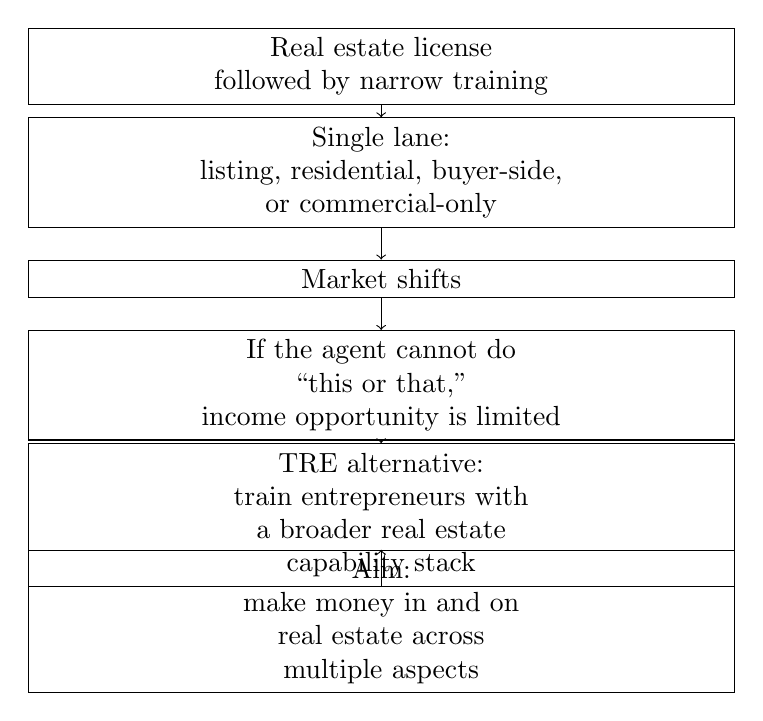
\begin{tikzpicture}[x=1cm,y=1cm]
\node[draw, align=center, text width=0.72\linewidth] (a) at (0,0)
{Real estate license\\followed by narrow training};
\node[draw, align=center, text width=0.72\linewidth] (b) at (0,-1.35)
{Single lane:\\listing, residential, buyer-side,\\or commercial-only};
\node[draw, align=center, text width=0.72\linewidth] (c) at (0,-2.70)
{Market shifts};
\node[draw, align=center, text width=0.72\linewidth] (d) at (0,-4.05)
{If the agent cannot do\\``this or that,''\\income opportunity is limited};
\node[draw, align=center, text width=0.72\linewidth] (e) at (0,-5.70)
{TRE alternative:\\train entrepreneurs with\\a broader real estate\\capability stack};
\node[draw, align=center, text width=0.72\linewidth] (f) at (0,-7.05)
{Aim:\\make money in and on\\real estate across\\multiple aspects};

\draw[->] (a) -- (b);
\draw[->] (b) -- (c);
\draw[->] (c) -- (d);
\draw[->] (d) -- (e);
\draw[->] (e) -- (f);
\end{tikzpicture}
\caption{A transcript-derived reconstruction of the speaker's mechanism: narrow training creates exposure to market shifts; capability stacking is presented as TRE's alternative.}
\end{figure}

The important feature of this diagram is its vertical order. We do not begin with an abstract theory of entrepreneurship. We begin with a license, then a narrow professional identity, then the risk of a market change, and only then the broader entrepreneurial model.

\section{Making Money In And On Real Estate}

The closing phrase is that TRE teaches entrepreneurs how to make money ``in and on'' real estate, and how to make money in every aspect of real estate. The phrase should be preserved because it is the speaker's own summary of the model.

A cautious reconstruction is
\begin{equation}
C_{\text{stack}}
\approx
C_{\text{in}}\cup C_{\text{on}},
\end{equation}
where \(C_{\text{in}}\) refers to capabilities inside the brokerage activity itself, and \(C_{\text{on}}\) refers to adjacent real estate activities such as investing or wholesaling. The symbol \(\approx\) is intentional. The transcript does not give a formal taxonomy of ``in'' versus ``on,'' so we should not pretend the boundary is exact.

In ordinary language, the speaker is asking us to stop treating real estate as one job. Listing, buying, residential, commercial, investing, and wholesaling are different channels through the same broad field. A person trained in only one channel is exposed to the fortunes of that channel. A person trained across several channels has more ways to interpret a deal, more ways to respond to a client, and more ways to adapt when the market changes.

\section{Summary}

The segment has a simple progression. First, the speaker describes the narrow path after a real estate license: the agent is taught to do one thing. Then he lists the roles and activities that often get separated from one another. TRE's pivot is to call its people entrepreneurs, meaning broader real estate professionals rather than one-lane agents.

The mechanism is market resilience. If income opportunity is written as \(I(m,C)\), then both the market \(m\) and the capability set \(C\) matter. The transcript does not supply numbers, probabilities, or a formal investment model. Its durable claim is more basic: when the market shifts, a single capability can become a ceiling, while a broader capability stack gives the entrepreneur more ways to make money in and on real estate.